% 09-mo-rong.tex — Chương 9: Khả năng áp dụng và mở rộng

\chapter{Khả năng áp dụng và mở rộng}\label{ch:morong}

\section{Mở rộng sang các bài toán khác}\label{sec:baitoankhac}

Phần đã xây dựng cho bài toán rời bỏ được tổ chức theo từng tầng độc lập nên nhiều tầng có thể tái sử dụng khi triển khai bài toán mới, thay vì làm lại từ đầu.

Các tầng nạp và kiểm tra dữ liệu, tạo chỉ số hành vi, huấn luyện và xét duyệt mô hình, chấm điểm, giám sát và đo hiệu quả bằng thử nghiệm đối chứng
đều có thể dùng lại; phần cần làm riêng cho mỗi bài toán mới là định nghĩa đáp án đúng, chỉ số bổ sung, thước đo chất lượng và đầu ra giao cho đơn vị sử dụng.

Mỗi bài toán mới sẽ được lập kế hoạch, đo lường và xét duyệt riêng trước khi vận hành, theo cùng nguyên tắc đã áp dụng cho bài toán rời bỏ.

\section{Khả năng áp dụng ngay cho bài toán rời bỏ}

{\tablefont
\begin{longtable}{@{}>{\bfseries}L{3.8cm}>{\raggedright\arraybackslash}p{11.83cm}@{}}
\caption{Các hướng áp dụng và mở rộng không cần thay đổi lớn}\label{tab:apdung}\\
\toprule
\hdrrow\hh{Hướng} & \hh{Cách thực hiện}\\
\midrule
\endfirsthead
\toprule
\hdrrow\hh{Hướng} & \hh{Cách thực hiện}\\
\midrule
\endhead
\bottomrule
\endfoot
Theo nhóm khách hàng & Điều chỉnh ngưỡng sản lượng, doanh thu, giá trị đơn trong bộ lọc điều kiện để tập trung vào nhóm giá trị cao, không phải sửa luồng xử lý.\\
\rowa Theo địa bàn, đơn vị quản lý & Dữ liệu đã có thông tin tỉnh và đơn vị quản lý hợp đồng; có thể cắt danh sách theo địa bàn để giao cho từng đơn vị chăm sóc.\\
Theo nguồn dữ liệu & Thêm nguồn mới bằng cách bổ sung cấu trúc nguồn và chỉ số tương ứng.\\
\rowa Theo mức ưu tiên & Điều chỉnh tỷ lệ cắt danh sách để phù hợp năng lực chăm sóc.\\
Theo lịch chạy & Tần suất nạp, huấn luyện, chấm điểm khai báo trong luồng công việc; có thể rút ngắn hoặc kéo dài.\\
\rowa Theo hạ tầng & Toàn bộ chạy bằng container, có thể chuyển sang máy chủ khác hoặc nền tảng điều phối lớn hơn.\\
\end{longtable}}
\vspace{4pt}

\section{Lộ trình nâng cấp bài toán rời bỏ}\label{sec:nangcap}

Các hướng sau không bắt buộc để hệ thống hiện tại hoạt động, nhưng giúp tăng độ tin cậy vận hành, khả năng kiểm soát và hiệu quả kinh doanh.

{\tablefont
\begin{longtable}{@{}L{3.5cm}>{\raggedright\arraybackslash}p{7.91cm}L{3.8cm}@{}}
\caption{Các hướng nâng cấp}\label{tab:nangcap}\\
\toprule
\hdrrow\hh{Hướng nâng cấp} & \hh{Nội dung} & \hh{Giá trị mang lại}\\
\midrule
\endfirsthead
\toprule
\hdrrow\hh{Hướng nâng cấp} & \hh{Nội dung} & \hh{Giá trị mang lại}\\
\midrule
\endhead
\bottomrule
\endfoot
Quản lý vòng đời mô hình & Ghi lại mỗi lần huấn luyện ; lưu mô hình trong registry với các nhãn ứng viên/đang dùng/dự phòng; chỉ chuyển khi qua cổng đánh giá. & Truy vết vì sao mô hình tháng này tốt hay xấu; quay lui nhanh\\
\rowa Kiểm tra dữ liệu định kỳ & Tự động báo cáo số dòng, tỷ lệ thiếu, phân phối chỉ số, tỷ lệ nhãn, số khách bị lọc theo từng lý do. & Phát hiện sớm dữ liệu bất thường\\
Kiểm tra lại trong quá khứ & Như Chương~\ref{ch:hieuqua}: giả lập vận hành tại nhiều mốc, đo theo tháng và theo nhóm. & Tin cậy vào kết quả, không dựa một lần kiểm tra\\
\rowa Thử nghiệm đối chứng & Như Chương~\ref{ch:hieuqua}. & Chứng minh giá trị kinh doanh\\
Giám sát trực quan  & Bảng điều khiển bốn nhóm: độ mới dữ liệu, chất lượng mô hình, kết quả chấm điểm, độ lệch; có cảnh báo chủ động. & Người điều hành xem sức khỏe hệ thống bằng biểu đồ\\
\rowa Điều phối thế hệ mới  & Mô hình hóa theo ``tài sản dữ liệu'' có phân vùng theo tháng, độ dài lịch sử; bù dữ liệu theo tháng dễ dàng. & Dễ truy nguồn gốc dữ liệu, giảm chạy sai thứ tự\\
Container hóa mức cao & Chạy các công việc nặng trên cụm máy, tách khỏi bộ lập lịch; quản lý tài nguyên, bí mật cấu hình. & Mở rộng quy mô, tăng tính sẵn sàng\\
\rowa Hợp đồng dữ liệu & Khai báo cấu trúc bắt buộc cho từng bảng nguồn; cảnh báo hoặc dừng khi thiếu cột, sai kiểu. & Giảm lỗi âm thầm khi nguồn đổi định dạng\\
\end{longtable}}
\vspace{4pt}

\begin{figure}[!ht]
\centering
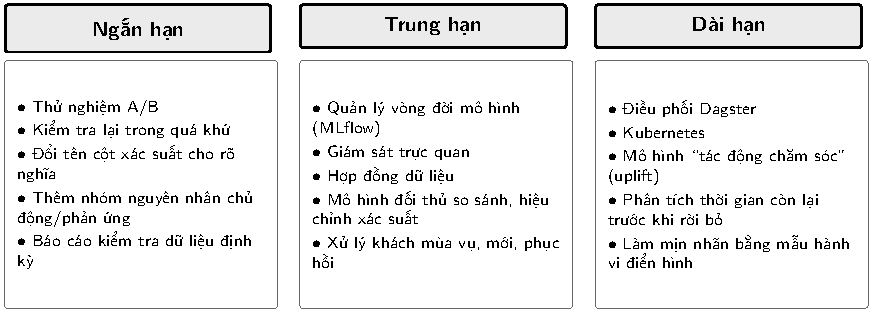
\includegraphics[width=418.9bp]{figures/fig11.pdf}
\caption{Gợi ý thứ tự triển khai các hướng nâng cấp, đề xuất của nhóm biên soạn}\label{fig:lotrinh}
\end{figure}

\section{Kỹ thuật phân tích có thể kết hợp}

{\tablefont
\begin{longtable}{@{}L{4.3cm}>{\raggedright\arraybackslash}p{11.33cm}@{}}
\caption{Các kỹ thuật bổ sung và khi nào nên dùng}\label{tab:kythuat}\\
\toprule
\hdrrow\hh{Kỹ thuật} & \hh{Khi nào nên dùng}\\
\midrule
\endfirsthead
\toprule
\hdrrow\hh{Kỹ thuật (nói đơn giản)} & \hh{Khi nào nên dùng}\\
\midrule
\endhead
\bottomrule
\endfoot
Thêm mô hình khác để so sánh  & Khi muốn tìm mô hình tốt hơn; dùng cùng dữ liệu, cùng cách chia thời gian để so sánh công bằng.\\
\rowa Hiệu chỉnh xác suất & Khi dùng điểm số như ``xác suất thật'' để tính doanh thu có nguy cơ mất, không chỉ để xếp hạng.\\
Phân tích thời gian còn lại & Khi cần trả lời ``khách này có thể rời bỏ sau bao lâu'', không chỉ ``có rời bỏ trong 2 tháng không''.\\
\rowa Mô hình tác động chăm sóc & Khi muốn tối ưu ngân sách: bỏ qua khách ``sẽ ở lại dù không chăm sóc'', tập trung khách ``chỉ giữ được nếu có can thiệp''.\\
Học theo chi phí & Khi cần phản ánh chi phí gọi nhầm và chi phí bỏ sót, hoặc doanh thu có nguy cơ mất, vào việc chọn ngưỡng.\\
\rowa Phát hiện bất thường & Khi quy tắc chưa bắt hết hình thái giảm đột ngột mới.\\
Mô hình chuỗi thời gian & Khi lịch sử đủ dài và ổn định, muốn học các kiểu diễn biến phức tạp.\\
\rowa Chỉ số theo bưu cục, tuyến, tỉnh & Khi chất lượng dịch vụ cục bộ ảnh hưởng đến việc rời bỏ.\\
Dự đoán đồng thời nhiều mục tiêu & Khi cần hành động cụ thể: dự báo cả rời bỏ, giảm đơn, giảm doanh thu, nhóm nguyên nhân.\\
Chỉ báo mức tin cậy & Khi cần chỉ tự động hành động ở nhóm có mức tin cậy cao, kiểm tra tay vùng sát ngưỡng.\\
\end{longtable}}
\vspace{4pt}

\section{Làm mịn nhãn bằng ``mẫu hành vi điển hình''}\label{sec:lamminh}

Hiện nay nhãn rời bỏ theo quy tắc là ``có'' hoặc ``không'' tuyệt đối. Với dữ liệu nghiệp vụ còn nhiễu, có thể làm mềm nhãn: xác định các mẫu hành vi điển hình xuất hiện trước khi khách rời bỏ, và các mẫu của khách ổn định, rồi dùng độ giống mẫu để điều chỉnh nhãn ở vùng quy tắc ``chưa chắc chắn''.

\begin{itemize}
  \item Các mẫu chỉ xây từ nhóm khách có độ tin cậy cao, và chỉ học trên phần dữ liệu học của từng vòng để tránh ``nhìn trộm''.
  \item Thực hiện ở nhánh thử nghiệm, so sánh với cách hiện tại trên bài thi cuối kỳ; không đưa vào vận hành nếu chỉ tăng F1 trên nhãn quy tắc mà không cải thiện kết quả ở thử nghiệm đối chứng.
\end{itemize}
